\documentclass[12pt,a4paper]{article}
\usepackage[warn]{mathtext}
\usepackage[utf8]{inputenc}
\usepackage[english,russian]{babel}
\usepackage{amsmath}
\usepackage{amssymb}
\usepackage{latexsym}
\usepackage{svg}
\usepackage{pgfplots}
\pgfplotsset{compat=1.9}

\usepackage{listings}

\usepackage{color}

\definecolor{dkgreen}{rgb}{0,0.6,0}
\definecolor{gray}{rgb}{0.5,0.5,0.5}
\definecolor{mauve}{rgb}{0.58,0,0.82}

\lstset{ %
	language=C++,                % Язык программирования 
	numbers=left,                   % С какой стороны нумеровать
	stepnumber=1,                   % Шаг между линиями. Если 1, то будет пронумерована каждая строка
	frame=single,	
}
\usepackage[left=2cm,right=2cm,
top=2cm,bottom=2cm,bindingoffset=0cm]{geometry}

\usepackage{sverb}
\usepackage{graphicx}
\usepackage{pdfpages}
\usepackage[absolute,overlay]{textpos}

\numberwithin{equation}{section}

\begin{document}
	\begin{titlepage}
		\begin{textblock*}{13cm}(0cm,0cm)
			
\includegraphics{reportTitle}
		\end{textblock*}
	\end{titlepage}
\hspace{0pt}
\clearpage
%	\begin{titlepage}
%		\centering
%		\Huge Лабораторная работа №1 по курсу \\\textbf{"Анализ алгоритмов"}\\
%		Тема: Расстояния Левенштейна и Дамерау-Левенштейна\\
%		\vspace{\baselineskip}
%		\Large Работу выполнил: Тюрин О.А. ИУ7-51Б\\
%		Преподаватели: Волкова Л.Л, Строганов Ю.В.
%		\vfill
%		Москва, 2020 г.		
%	\end{titlepage}
\tableofcontents
\clearpage

\addcontentsline{toc}{section}{Введение}
%//////////////////////////////////////////////////////////////////
\section*{\Huge Введение}
\qquad На данный момент существует огромной количество сортировок, именно поэтому их необходимо уметь сравнивать для того, чтобы выбрать наиболее подходящий для конкретного случая алгоритм.\\\\
{Цель работы:} оценить трудоемкость алгоритмов сортировки массива и получить практический навык реализации алгоритмов.\vspace{\baselineskip} 

{Задачи работы:}
\begin{enumerate}
	\item изучить алгоритмы сортировки массива: пузырьком, выбором и \textit{quick sort}; 
	\item оценить трудоемкость данных алгоритмов сортировки;
	\item реализовать данные алгоритмы сортировки массива на одном из языков программирования;  
	\item сравнить рассматриваемые алгоритмы сортировки между собой.
\end{enumerate}

\qquad Алгоритмы сортировки оцениваются по следующим критериям:
\begin{itemize}
	\item затрачиваемое время;
	\item затрачиваемая память.
\end{itemize}

\clearpage

\section{Аналитическая часть}
\qquad Сортировка - это процесс упорядочивания наборов данных одного типа по возрастанию или убыванию значения какого-либо признака.\\
\textbf{Области применения сортировки:} 
\begin{itemize}
	\item анализ данных;
	\item физика;
	\item экономика.
\end{itemize}

\subsection{Описание алгоритмов}
\qquad В данном разделе будут описан каждый исследуемый алгоритм.

\subsection{Сортировка пузырьком}
\qquad Алгоритм проходит по массиву {n-1} раз или до тех пор, пока массив не будет полностью отсортирован. 
В каждом проходе элементы попарно сравниваются и, при необходимости, меняются местами.
При каждом проходе алгоритма по внутреннему циклу, очереднй наибольший элемент ставится на своё место в конец неотсортированного массива. 
Таким образом наибольшие элементы "всплывают" как пузырек. 

\subsection{Сортировка выбором}
\qquad Берётся первый элемент массива, далее происходит трассировка оставшегося массива в поисках наименьшего числа. Когда мы пробегаем весь массив, если меньшее число найдено — меняем его местами с первым элементом. После этого берётся второй элемент, и все повторяется, пока для каждого элемента мы не будет пройдена оставшаяся часть массива.

\subsection {Быстрая сортировка}
\qquad Массив разбивается на два (возможно пустых) подмассива. Таких, что в одном подмассиве каждый элемент меньше либо равен опорному, 
и при этом не превышает любой элемент второго подмассива. Опорный элемент вычислыется в ходе процедуры разбиения. 
Подмассивы сортируются с помощью рекурсивного вызова процедуры быстрой сортировки. 
Поскольку подмассивы сортируются на месте, для их объединения не трубуются никакие действия.

\addcontentsline{toc}{subsection}{Вывод}
\section*{Вывод}
\qquad В данном разделе было приведено описание работы каждого из алгоритмов.
\clearpage

\section{Конструкторская часть}
\textbf{Требования к вводу:} на вход подаются размерность массива и сам массив чисел.\\\\
\textbf{Требования к программе:}:\\
\begin{itemize}
\item корректная сортировка массива;
\item программа должна корректно обрабатывать массивы нулевой размерности.
\end{itemize}
\clearpage
\subsection{Разработка алгоритмов} % Сюда схемы алгоритмов
В данном разделе представлены схемы реализуемых алгоритмов.

На рисунке 2.1 представлена схема алгоритма сортировки пузырьком.\\
\begin{center}	
	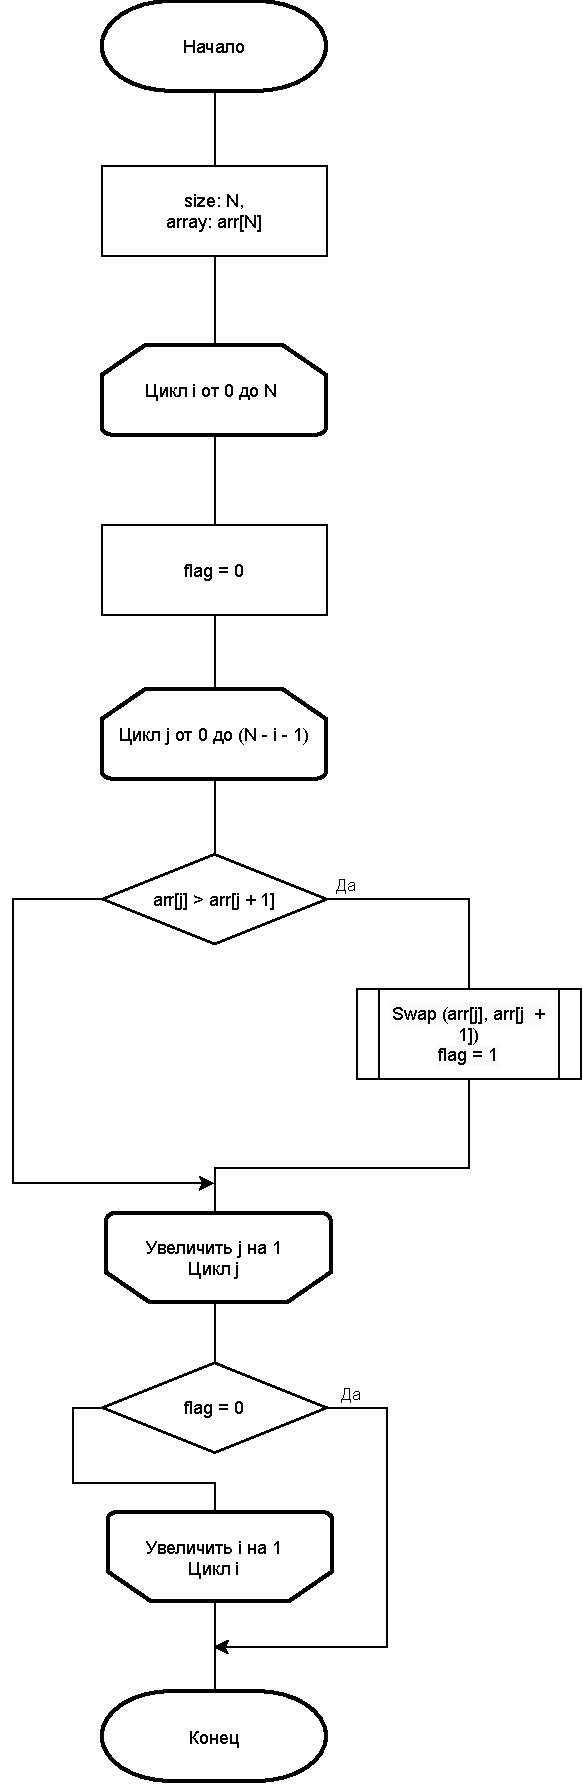
\includegraphics[width=.4\linewidth]{src/schemas/bubbleSort}\\
	Рис. 2.1: Схема алгоритма сортировки пузырьком
\end{center}
\clearpage
На рисунке 2.2 представлена схема алгоритма сортировки выбором.\\
\begin{center}	
	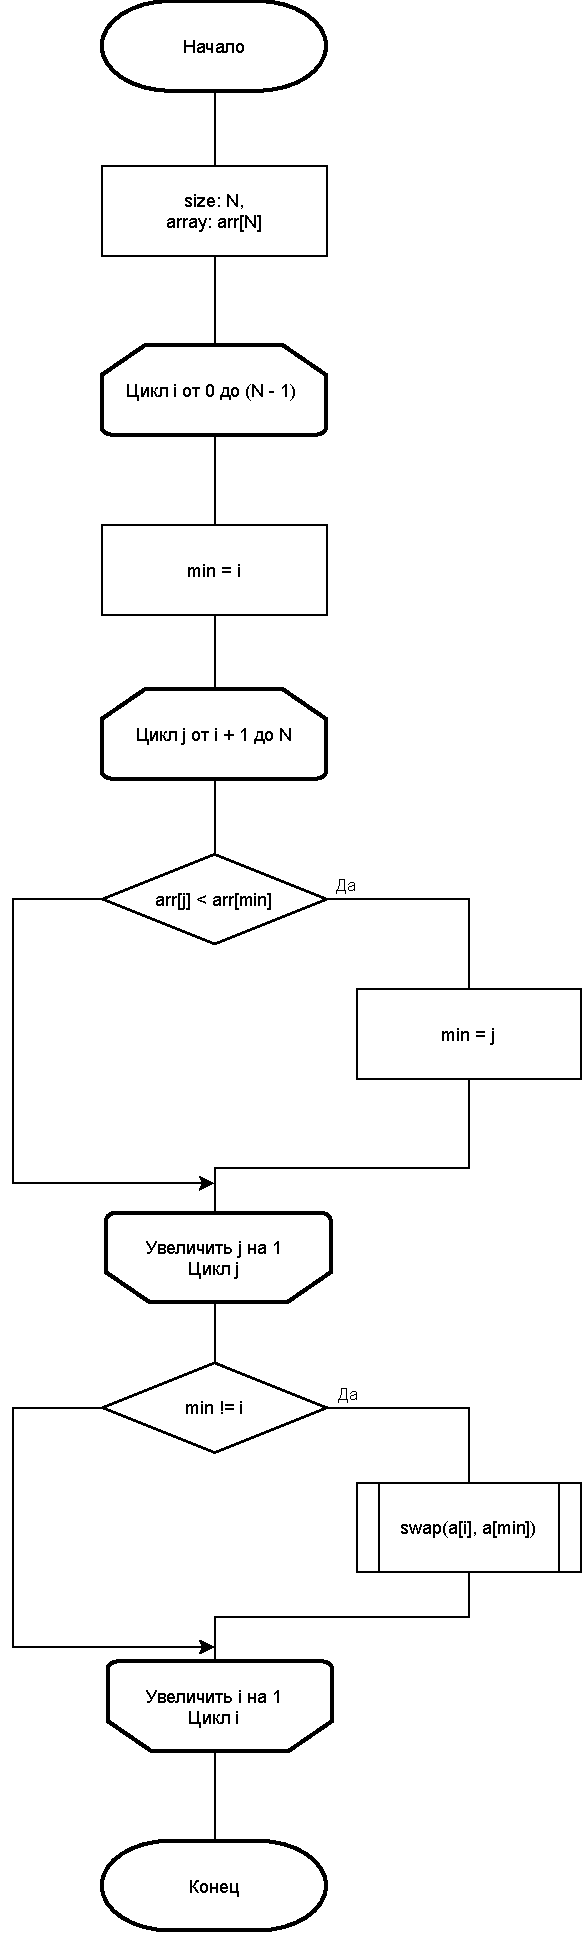
\includegraphics[width=.4\linewidth]{src/schemas/ShellSort}\\
	Рис. 2.2: Схема алгоритма сортировки Выбором
\end{center}
\clearpage
На рисунке 2.3 представлена схема алгоритма быстрой сортировки.\\
\begin{center}
	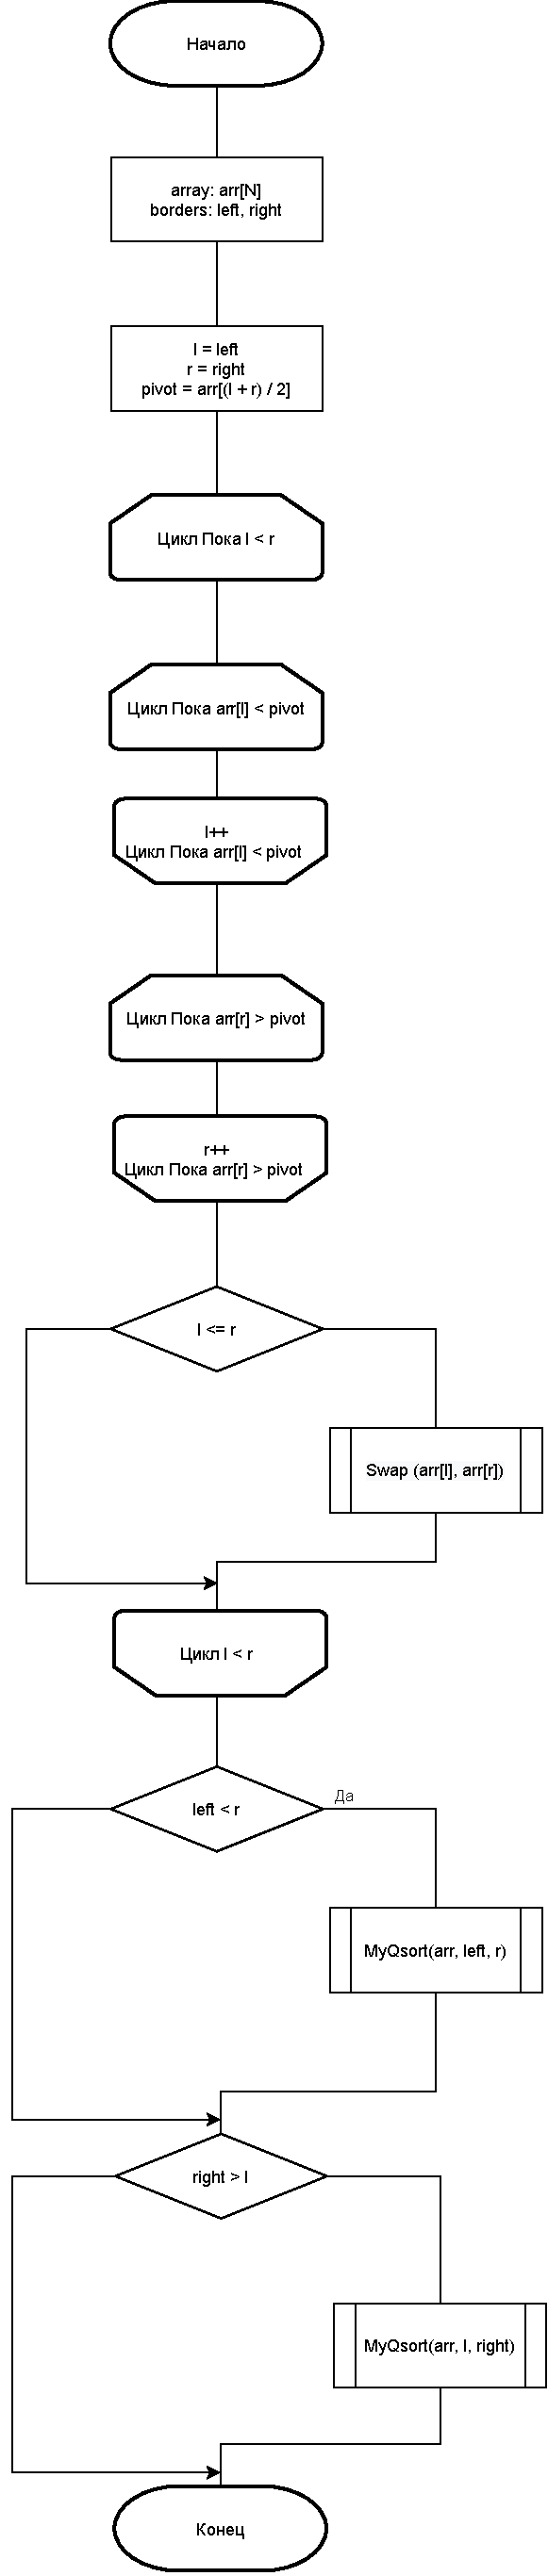
\includegraphics[width=.3\linewidth]{src/schemas/QSort}\\
	Рис. 2.3: Схема алгоритма быстрой сортировки
\end{center}
\clearpage
\addcontentsline{toc}{subsection}{Вывод}
\section*{Вывод}
\qquad В данном разделе были рассмотрены схемы реализуемых алгоритмов.
\clearpage

\section{Технологическая часть}
\qquad В данном разделе будет описана технологическая часть лабораторной работы: требования к ПО, листинг кода, сравнительный анализ всех алгоритмов.
\subsection{Требования к программному обеспечению}
Входные данные: размерность массива, сам массив\\
Выходные данные: отсортированный массив\\
Среда выполнения: Windows 10 x64
\subsection{Средства реализации}
\qquad Для выполнения данной работы был использован Python 3.9.0
\subsection{Листинг кода}
\qquad В данном разделе будет представлен листинг кода разработанных алгоритмов.\\

Ниже, на листинге 3.1, представлена реализация алгоритма сортировки пузырьком:
\begin{center}
	Листинг 3.1: Сортировка пузырьком
	\lstinputlisting[language=C++]{src/code/bubbleSort.cpp}
\end{center}
\clearpage

Ниже, на листинге 3.2, представлена реализация алгоритма сортировки выбором:
\begin{center}
	Листинг 3.2: Сортировка выбором
	\lstinputlisting[language=C++]{src/code/selectionSort.cpp}
\end{center}

Ниже, на листинге 3.3, представлена реализация алгоритма быстрой сортировки:
\begin{center}
	Листинг 3.3: Быстрая сортировка
	\lstinputlisting[language=C++]{src/code/QSort.cpp}
\end{center}
\clearpage

\subsection{Трудоемкость алгоритмов}
\qquad Введем модель трудоемкости для оценки алгоритмов:\\
\begin{itemize}
\item базовые операции стоимостью 1: +, -, *, /, =, ==, <=, >=, !=, +=, [], получение полей класса (в том числе и геттеры);
\item оценка трудоемкости цикла: $F_{cycle} = init +  N*(statement + iteration + F_{body}) + statement$, где init - инициализация цилка, N - количество итераций цикла, iteration - действие в конце каждой итерации цикла, statement - выражение, описывающее условие цикла;
\item стоимость условного перехода применим за 0, стоимость вычисления; условия остаётся.
\end{itemize}
	
\subsubsection{Трудоёмкость алгоритма сортировки пузырьком}
\qquad Рассмотри трудоёмкость алгоритма сортировки пузырьком.\\
Лучший случай: массив изначально отсортирован. Был сделан один проход, в ходе которого было установлено, что массив уже отсортирован\\
\begin{equation}
	1 + 1 + 1 + 1 + 1 + (size - 1)(3 + 1 + 4) + 3 + 1\\
\end{equation}
\begin{equation}
8*(size) + 1 = O(n)\\
\end{equation}

Худший случай: массив отсортирован в обратном порядке\\
\begin{equation}
	1 + 1 + size*(1 + 1 + 1 + 1 + (size - 1)(2 + 1 + 4 + 1 + 3) + 2) + 1\\
\end{equation}
\begin{equation}
	11*size*size - 5*size + 3 = O(n^2)\\
\end{equation}

\subsubsection{Трудоёмкость алгоритма сортировки выбором}
\qquad Рассмотри трудоёмкость алгоритма сортировки выбором.\\
Лучший случай: массив изначально отсортирован.\\
\begin{equation}
	1 + 1 + (size - 1)(2 + 1 + 1 + 2 + (size - i - 1)(3) + 1 + 1) + 2\\
\end{equation}

\begin{equation}
	3*size*size + ... = O(n^2)\\
\end{equation}
Как видно, даже в самом лучшем случае сложность квадратичная.\\

Худший случай: массив отсортирован в обратном порядке\\
\begin{equation}
	1 + 1 + (size - 1)(2 + 1 + 1 + 2 + (size - i - 1)(3) + 1 + 3 + 1) + 2\\
\end{equation}

\begin{equation}
	3*size*size + ... = O(n^2)\\
\end{equation}


\subsubsection{Трудоёмкость алгоритма быстрой сортировки}
\qquad Рассмотрим трудоёмкость алгоритма быстрой сортировки.\\
Лучший случай: Разбиение на подмассивы происходит таким образом, что их размерности совпадают, либо разлчиаются на 1. При таком раскладе глубина рекурсии будет равняться $log(size)$. В любом случае нам необходимо будет сравнить все элементы массива. Таким образом сложность равна:\\
\begin{equation}
	O(size * log(size))\\
\end{equation}


\qquad Худший случай: Разбиение на подмассивы происходит таким образом, что их размерность одного из подмассивов равен 1 (т.е. на каждом из этапов в качестве pivot был выбран либо наименьший, либо наибольший из обрабатываемых элементов). При таком раскладе глубина рекурсии будет равняться $n$. В любом случае нам необходимо будет сравнить все элементы массива. Таким образом сложность равна:\\
\begin{equation}
O(n^2)\\
\end{equation}




\subsection{Описание тестирования} % описать, какие тесты будут проведены ВСЕ ТЕСТЫ ПРОЙДЕНЫ УСПЕШНО
Были проведены следующие тривиальные тесты:\\
\begin{lstlisting}
arr = [10, -1, 0 ,4, 5, 8]

Bubble sort: [10, -1, 0 ,4, 5, 8]

Selection sort: [10, -1, 0 ,4, 5, 8]

Quick sort: [10, -1, 0 ,4, 5, 8]

\end{lstlisting}

\qquad Также были проведены тесты на больших размерностях со случайными числами в качестве элементов. В качестве эталона для сравнения массивов была использована функция sorted.\\
\qquad Ниже, на листинге 3.4, представлен фрагмент кода тестирования корректной работы реализации алгоритмов
\begin{center}
	Листинг 3.4: Тестирование корректной работы алгоритмов
	\lstinputlisting[language=C++]{src/code/tests.cpp}	
\end{center}

Все тесты пройдены успешно.

\addcontentsline{toc}{subsection}{Вывод}
\section*{Вывод}
\qquad В данном разделе был представлен листинг реализованных алгоритмов, а также описание тестирование корректности их работы.
\clearpage

\section{Экспериментальная часть}
\qquad В данной части работы будут приведен анализ алгоритмов на основе эксперементальных данных.
\subsection{Сравнительный анализ на основе замеров времени работы алгоритмов}
\qquad Был проведён замер времени работы каждого из алгоритмов. Каждый эксперимент на каждой размерности был произведён 10 раз, затем бралось среднее арифметическое полученного результата.\\
\qquad Все эксперименты были проведены для размерностей, начиная со 100, заканчивая 1000 с шагом 100.\\
\qquad Ниже во всех таблицах время сортировки указано в миллисекундах.\\
\qquad Ниже, в таблице 4.1, представлена таблица замеров времени работы алгоритмов.\\
\qquad Ниже, на графиках 4.1.1 и 4.1.2, представлена графическая интерпретация\\
\subsubsection{Эксперимент 1}
\qquad Массив отсортирован
\begin{center}
	Таблица 4.1: Замеры времени работы алгоритмов
	\begin{tabular}{| l | | l | l | l |}
		\hline
		Размерность & Bubble & Selection & QSort\\\hline
		100  & 0.00075 & 0.0365  & 0.00335 \\\hline
		200  & 0.00129 & 0.12175 & 0.00684 \\\hline
		300  & 0.00186 & 0.28013 & 0.01037 \\\hline
		400  & 0.00289 & 0.46373 & 0.01369 \\\hline
		500  & 0.00281 & 0.69324 & 0.02068 \\\hline
		600  & 0.00366 & 1.18182 & 0.0247 \\\hline
		700  & 0.00404 & 1.64755 & 0.03094 \\\hline
		800  & 0.00495 & 2.02626 & 0.0384 \\\hline
		900  & 0.00515 & 2.47341 & 0.04203 \\\hline
		1000 & 0.00697 & 2.87887 & 0.04861\\\hline
	\end{tabular}
\end{center}

\begin{center}
	График 4.1.1: Замеры вермени работы алгоритмов\\
	\begin{tikzpicture}
	\begin{axis}
	\addplot coordinates {
		(100, .00075) (200, .00129) (300, .00186) (400, .00289) (500, .00281) (600, .00366) (700, .00404) (800, .00495) (900, .00515) (1000, .00697)
	};
	\addplot coordinates {
		(100, 0.0365) (200, 0.12175) (300, 0.28013) (400, 0.46373) (500, 0.69324) (600, 1.18182) (700, 1.64755) (800, 2.02626) (900, 2.47341) (1000, 2.87887)
	};
	\addplot coordinates {
		(100, 0.00335) (200, 0.00684) (300, 0.01037) (400, 0.01369) (500, 0.02068) (600, 0.0247) (700, 0.03094) (800, 0.0384) (900, 0.04203) (1000, 0.04861)
	};
	\end{axis}
	\end{tikzpicture}
	\\
	Легенда:\\
	Синий цвет - Сортировка пузырьком\\
	Красный цвет - Сортировка выбором\\
	Коричневый цвет - Быстрая сортировка\\
	
	График 4.1.2: Замеры вермени работы алгоритмов\\
	\begin{tikzpicture}
	\begin{axis}
	\addplot coordinates {
		(100, .00075) (200, .00129) (300, .00186) (400, .00289) (500, .00281) (600, .00366) (700, .00404) (800, .00495) (900, .00515) (1000, .00697)
	};
	\addplot coordinates {
		(100, 0.00335) (200, 0.00684) (300, 0.01037) (400, 0.01369) (500, 0.02068) (600, 0.0247) (700, 0.03094) (800, 0.0384) (900, 0.04203) (1000, 0.04861)
	};
	\end{axis}
	\end{tikzpicture}
	\\
	Легенда:\\
	Синий цвет - Сортировка пузырьком\\
	Красный цвет - Быстрая сортировка\\
\end{center}
\subsubsection{Эксперимент 2}
Массив отсортирован в обратном порядке\\
Ниже, в таблице 4.2, представлена таблица замеров времени работы алгоритмов.\\
Ниже, на графике 4.2, представлена графическая интерпретация\\
\begin{center}
	Таблица 4.2: Замеры времени работы алгоритмов
	\begin{tabular}{| l | | l | l | l |}
		\hline
		Размерность & Bubble & Selection & QSort\\\hline
		100 & 0.10772 & 0.03127 & 0.00349\\\hline 
		200 & 0.82298 & 0.28794 & 0.01623\\\hline
		300 & 1.95633 & 0.453 & 0.01292\\\hline
		400 & 1.48573 & 0.45165 & 0.01531\\\hline
		500 & 2.59618 & 1.1219 & 0.01746\\\hline
		600 & 2.92382 & 0.91247 & 0.02086\\\hline
		700 & 3.73524 & 1.16877 & 0.02568\\\hline
		800 & 5.24454 & 1.53452 & 0.02697\\\hline
		900 & 6.2039 & 1.92548 & 0.02995\\\hline
		1000 & 7.8126 & 2.40036 & 0.0319\\\hline
	\end{tabular}
\end{center}
\begin{center}
	График 4.2: Замеры вермени работы алгоритмов\\
	\begin{tikzpicture}
	\begin{axis}
	\addplot coordinates {
		(100, 0.10772) (200, 0.82298) (300, 1.95633) (400, 2.17621) (500, 2.59618) (600, 2.92382) (700, 3.73524) (800, 5.24454) (900, 6.2039) (1000, 7.8126)
	};
	\addplot coordinates {
		(100, 0.03127) (200, 0.28794) (300, 0.453) (400, 0.45165) (500, 0.76077) (600, 0.91247) (700, 1.16877) (800, 1.53452) (900, 1.92548) (1000, 2.40036)
	};
	\addplot coordinates {
		(100, 0.00349) (200, 0.01623) (300, 0.01292) (400, 0.01531) (500, 0.01746) (600, 0.02086) (700, 0.02568) (800, 0.02697) (900, 0.02995) (1000, 0.03192)
	};
	\end{axis}
	\end{tikzpicture}
	\\
	Легенда:\\
	Синий цвет - Сортировка пузырьком\\
	Красный цвет - Сортировка выбором\\
	Коричневый цвет - Быстрая сортировка\\
\end{center}
\subsubsection{Эксперимент 3}
\qquad Массив заполнен случайными значениями
\qquad Ниже, в таблице 4.3, представлена таблица замеров времени работы алгоритмов.\\
\qquad Ниже, на графике 4.3, представлена графическая интерпретация\\
\begin{center}
	Таблица 4.3: Замеры времени работы алгоритмов
	\begin{tabular}{| l | | l | l | l |}
		\hline
		Размерность & Bubble & Selection & QSort\\\hline
		100 & 0.00438 & 0.00539 & 0.00563\\\hline
		200 & 0.70537 & 0.13577 & 0.01681\\\hline
		300 & 1.09619 & 0.26728 & 0.02833\\\hline
		400 & 1.81696 & 0.54301 & 0.04036\\\hline
		500 & 2.11177 & 0.78962 & 0.06112\\\hline
		600 & 2.64796 & 0.95799 & 0.05681\\\hline
		700 & 3.41683 & 1.1714 & 0.0715\\\hline
		800 & 4.55442 & 1.52958 & 0.08578\\\hline
		900 & 5.82487 & 2.17994 & 0.09873\\\hline
		1000 & 7.04937 & 2.44209 & 0.11722\\\hline
	\end{tabular}
\end{center}
\begin{center}
	График 4.3: Замеры вермени работы алгоритмов\\
	\begin{tikzpicture}
	\begin{axis}
	\addplot coordinates {
		(100, 0.00438) (200, 0.70537) (300, 1.09619) (400, 1.81696) (500, 2.11177) (600, 2.64796) (700, 3.41683) (800, 4.55442) (900, 5.82487) (1000, 7.04937)
	};
	\addplot coordinates {
		(100, 0.00539) (200, 0.13577) (300, 0.26728) (400, 0.54301) (500, 0.78962) (600, 0.95799) (700, 1.1714) (800, 1.52958) (900, 2.17994) (1000, 2.44209)
	};
	\addplot coordinates {
		(100, 0.00563) (200, 0.01681) (300, 0.02833) (400, 0.04036) (500, 0.06112) (600, 0.05681) (700, 0.0715) (800, 0.08578) (900, 0.09873) (1000, 0.11722)
	};
	\end{axis}
	\end{tikzpicture}
	\\
	Легенда:\\
	Синий цвет - Сортировка пузырьком\\
	Красный цвет - Сортировка выбором\\
	Коричневый цвет - Быстрая сортировка\\
\end{center}
\subsection{Сравнительный анализ на материале экспериментальных данных}
\qquad В результате экспериментов было выявлено, что теоретичесие расчёты сложности верны. В лучшем случае сортировка пузырьком имеет линейное время, а сортировка выбором - квадратичное. Но в то же время в худшем случае оба алгоритма имеют одинаковую сложность - квадратичную. Однако сортировка пузырьком имеет больший  коэфициент при квадрате, следовательно, и работает она медленнее. В то же время быстрая сортировка прекрасна показала себя во всех экспериментах.
\addcontentsline{toc}{subsection}{Вывод}
\section*{Вывод}
\qquad В данном разделе были представлены эксперименты, проведённые над реализованным алгоритмами.
\clearpage
\addcontentsline{toc}{section}{Заключение}
\section*{\Huge Заключение}
\qquad В ходе работы были изучены  и реализованы следующие алгоритмы сортировки: пузырьковая сортировка, сортировка выбором и быстрая сортировка. Была дана теоретическая оценка всех рассматриваемых алгоритмов, было проведено тестирование и выполнено сравнение всех рассматриваемых алгоритмов. В ходе исследования была установлена зависимость времени выполнения алгоритмов от изначального заполнения массивов.

%//////////////////////////////////////////////////////////////////
\clearpage
\renewcommand\refname{Список использованной литературы}
\begin{thebibliography}{}
	\bibitem{academy} Основные виды сортировок и примеры их реализации. [электронный ресурс]. Режим доступа: https://academy.yandex.ru/posts/osnovnye-vidy-sortirovok-i-primery-ikh-realizatsii
	(Дата обращения: 16.10.2020)
	
	\bibitem{habr} Описание алгоритмов сортировки и сравнение их производительности [электронный ресурс]. Режим доступа:
	https://habr.com/ru/post/335920/, свободный
	(Дата обращения: 16.10.2020)
	
	\bibitem{time} Официальный сайт Python, документация [электронный ресурс]. Режим доступа: https://docs.python.org/3/library/time.html, свободный (Дата обращения: 16.09.20)
\end{thebibliography}
\end{document}